\section{Существующие решения}

В этом разделе будут рассмотрены существующие программные продукты, позволяющие разработчикам интегрировать в свои приложения возможности расширения либо автоматизации. Особое внимание уделено продуктам, совместимым с платформой {\it .NET}, так как в работе речь будет идти именно о ней.

Так же в этой главе будут рассмотрены продукты, не имеющие совместимости с платформой {\it .NET}, однако представляющие ценность для данного исследования, как хорошо зарекомендовавшие себя на рынке ПО для автоматизации приложений. Ярким примером такого ПО является {\it VBA (Visual Basic for Applications)}.

Кроме того, некоторое внимание будет уделено технологиям, языкам программирования, библиотекам, которые решают поставленные задачи частично, либо вообще не решают их, но которые интересны с точки зрения возможности из применения рамках проекта по созданию платформы для расширения и автоматизации ПО.

\subsection{Автоматизация}

\subsubsection{Visual Basic for Applications}

{\it Visual Basic for Applications} -- разработка компании {\it Microsoft}, совмещающая в себе реализацию языка программирования {\it Visual Basic} и соответствующую среду разработки~\cite{mastering-vba}. {\it VBA} является интерпретируемым языком: исходный код программы компилируется в промежуточный {\it P-код}, который впоследствии выполняется виртуальной машиной, являющейся частью основного приложения. {\it VBA} построен на технологии {\it COM}, благодаря чему {\it VBA-}код может использовать все доступные в операционной системе {\it COM}-объекты и компоненты {\it ActiveX}. Интегрированная среда разработки предоставляет удобный редактор кода с подсветкой синтаксиса и системой автодополнения кода, набор инструментов для удобной работы с проектами и файлами исходного кода, а также отладчик. Одно из важных достоинств {\it VBA} -- сравнительная лёгкость освоения.

Изначально {\it VBA} был встроен в семейство продуктов {\it Microsoft Office}. Из кода макроса на {\it VBA} пользователь может получить доступ ко всем функциям, доступным через графический интерфейс пользователя, а также к многочисленным функциям операционной системы и компонентов сторонних разработчиков.

Помимо {\it Microsoft Office} {\it VBA} встроен во многие программные продукты других разработчиков, к примеру,  {\it AutoCAD}, {\it SolidWorks}, {\it CorelDRAW}, {\it WordPerfect} и {\it ESRI ArcGIS}. Более того, {\it VBA} можно использовать при разработке любого {\it Windows}-приложения для внедрения в него возможности автоматизации. 

В настоящее время технология {\it VBA} считается устаревшей и более не поддерживается. В качестве замены {\it Microsoft} предлагает технологии {\it VSTA}~\cite{vsta-website} и {\it VSTO}~\cite{vsto-website}, речь о которых пойдёт в следующих разделах.
\subsection{Visual Studio Tools for Applications}

{\it Visual Studio Tools for Applications (VSTA)} -- это набор инструментов, который независимые поставщики программного обеспечения могут использовать для добавления возможностей автоматизации и расширения в свои приложения. {\it VSTA} был объявлен {\it Microsoft} с выпуском интегрированной реды разработки {\it Visual Studio 2005}. {\it VSTA} основана на платформе {\it .NET Framework} и построена на той же архитектуре, что и {\it VSTO}, речь о которой пойдёт в следующем разделе. {\it VSTA} включает в себя интегрированную среду разработки, являющуюся упрощённой версией IDE {\it Visual Studio}. Основные языки программирования, используемые в {\it VSTA} -- это {\it Visual Basic .NET} и {\it C\#}, однако в общем случае может быть использован любой язык для платформы {\it .NET}. Благодаря тесной интеграции с {\it .NET} пользовательский код имеет доступ ко всей библиотеке классов этой платформы, что существенно расширяет спектр возможностей при написании расширений и макросов. Важной особенностью {\it VSTA} является поддержка 64-битной архитектуры. 

Платформа {\it VSTA} распространется бесплатно, однако разработчики, планирующие включать {\it VSTA} в состав коммерческого приложения, должны приобрести соответствующую лицензию.
\subsubsection{Visual Studio Tools for Office}

{\it Visual Studio Tools for Office} -- это набор средств разработки, доступных в виде расширений {\it Visual Studio} (шаблонов проектов) и исполняющей среды, позволяющей  семейству продуктов {\it Microsoft Office} 2003 и более поздних версий загружать и выполнять пользовательский код {\it .NET} для расширения функциональности приложений {\it Office} и их автоматизации~\cite{vsto-website}. {\it VSTO} пришла на замену технологии {\it VBA}, использующейся в более ранних версиях {\it Microsoft Office}. 

Расширения {\it VSTO} разрабатываются в интегрированной среде {\it Visual Studio}. Пользовательский код имеет доступ ко всей библиотеке классов {\it .NET}. Как и в случае с {\it VBA}, макрос выполняется виртуальной машиной (в данном случае - CLR, Common Language Runtime), которая работает в рамках процесса основного приложения. Но в отличие от {\it VBA} код сохраняется в отдельной сборке {\it .NET}.
\subsubsection{Другие разработки}

Помимо универсальных платформ для автоматизации, рассмотренных выше, существует множество скриптовых языков, которые могут быть использованы для создания собственной платформы, решающей задачи автоматизации ПО. Некоторые из этих языков (как правило, речь идет о диалектах языка, нацеленных на эффективную работу с одним из программных продуктов) разрабатывались специально для конкретной задачи по автоматизации приложения. Это позволило глубоко интегрировать скриптовый язык в архитектуру приложения, которое он расширяет. Яркими примерами такогих языков являются диалекты языка Lisp. AutoLisp с 1986 года применяется в AutoCAD и неразрывно с ним связан, Emacs Lisp используется в текстовых редакторах GNU Emacs и XEmacs. Особенностью таких узкоспециализированных скриптовых языков является глубокая интеграция с приложением и сложность в освоении. Они хорошо подходят для решения задач, специфичных для конкретного приложения, но их использование как универсального инструмента для автоматизации ПО невозможно.

Так же существует несколько скриптовых языков, совместимых с платформой .NET. Наиболее перспективным и популярным из них является IronPython, на примере которого и будет рассмотрена концепция использования скриптового языка для автоматизации основного приложения.


\subsubsection{IronPython} % TODO :: перенести в отдельный файл?
{\it IronPython} -- реализация языка программирования {\it Python} для платформ {\it .NET Framework} и {\it Mono}. {\it IronPython} полностью написан на {\tt C\#}, и является транслятором компилирующего типа. Код скрипта, написанного на {\it IronPython}, может использоваться одним из следующих способов:
\begin{itemize}
 \item посредством компиляции в независимую сборку, которая в дальнейшем может быть загружена в приложение как зависимось или с помощью {\it .NET Reflection};
 \item посредством размещения {\it IronPython}-подсистемы в основном приложении и динамической трансляции кода.
\end{itemize}

Эта особенность {\it IronPython} очень важна в контексте задач, связанных с автоматизацией ПО.

На схеме ниже рассмотрен типичный способ использования {\it IronPython} с целью автоматизации приложения:

\TODO{ (dennis.yolkin) схема и её описание}.
\subsubsection{IronPython}

{\it IronPython} -- реализация языка программирования {\it Python} для платформ {\it .NET Framework} и {\it Mono}. {\it IronPython} полностью написан на {\tt C\#}, и является транслятором компилирующего типа. Код скрипта, написанного на {\it IronPython}, может использоваться одним из следующих способов:
\begin{itemize}
 \item посредством компиляции в независимую сборку, которая в дальнейшем может быть загружена в приложение как зависимось или с помощью {\it .NET Reflection};
 \item посредством размещения {\it IronPython}-подсистемы в основном приложении и динамической трансляции кода.
\end{itemize}

Эта особенность {\it IronPython} очень важна в контексте задач, связанных с автоматизацией ПО.

На схеме, представленной на рисунке \ref{ironpython-scheme}, рассмотрен типичный способ использования {\it IronPython} с целью автоматизации приложения, разрабатываемого для платформы .NET:

\begin{figure}[!h]
    \centering
    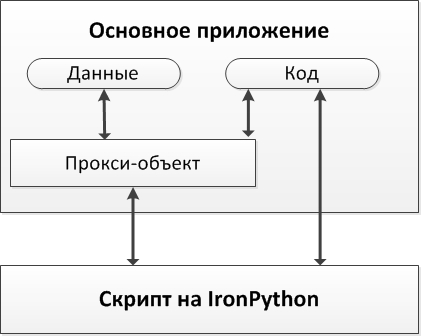
\includegraphics[width=9cm]{ironpython1.jpg}
    \caption{Взаимодействие хост-приложения и скрипта на IronPython}
    \label{ironpython-scheme}
\end{figure}

Для обеспечения взаимодействия скрипта и основного приложения создаётся прокси-объект. Фактически, в этом объекте содержатся ссылки на данные, к которым может осуществляться доступ из скрипта. Теоретически возможен примой доступ к публичным данным хост-приложения, но использовать такую модель не рекомендуется из соображений безопасности и соответствия основным парадигмам объектно-ориентированного приложения. Помимо данных, скрипт может использовать код (классы и функции), реализованный в хост-приложении.

\subsubsection{Выводы}

Из краткого обзора существующих продуктов для автоматизации видно, что только компания Microsoft предлагает универсальные решения, готовые к интеграции <<из коробки>> и подходящие большинству разработчиков. И в случае разработки собственной платформы имеет смысл ориентироваться на функциональность продуктов этой компании. Особого внимания для реализации поставленной задачи заслуживает набор инструментов {\it VSTA}, так как является наследником используемого в исходном продукта {\it VBA}. {\it VSTA} имеет необходимый набор возможностей и, согласно документации, позволяет использовать различные сценарии интеграции в расширяемое приложение.

\subsection{Расширение}

\subsubsection{MEF (Microsoft Extensibility Framework)}

{\it MEF} -- библиотека для создания расширяемых приложений. Она позволяет разработчикам программного обеспечения исползовать расширения без необходимости дополнительного конфигурирования. Благодаря {\it MEF}, исходный код расширения полностью независим и не возникает проблем с сильной связностью компонентов приложения и расширения. С помощью {\it MEF} можно разрабатывать как расширения для конкретного приложения, так и универсальные расширения, которые могут быть интегрированны в самые различные продукты.

Обычно в основе любой системы плагинов лежит некий общий интерфейс, который должен быть реализован любым расширением. Интерфейс описывает способы взаимодействия основного приложения и расширения. Это накладывает дополнительное ограничение, добавляя лишнюю зависимость между приложением и плагином. Помимо этого, никаки не регламентируется способ взаимодействия между различными плагинами. Ситуация, в которой один плагин зависит от набора других плагинов (и может функционировать только если разрешены все зависимости), в общем случае оказывается неразрешимой.

Подход, выбранный разработчиками {\it MEF} направлен в первую очередь на упрощение разрешения зависимостей между основным приложением и расширением и между различными расширениями.

Вместо необходимости явной регистрации доступных компонентов-расширений, {\it MEF} предоставляет возможность автоматически неявно обнарруживать подходящие расширения. Любое расширение в {\it MEF} декларативно описывает все свои зависимости (в терминах платформы - {\tt imports}) и предоставляемые возможности ({\tt exports}).

Такое решение решает проблемы с зависимостями, описанные ранее. Раз зависимости и предоставляемый функционал описывается декларативно, любое расширение может быть <<подключено>> к основному приложению в процессе выполнения (без перезапуска приложения и тем более без перекомпиляции исходного кода). Таким образом, нет жёстких зависимостей между расширением и расширяемым приложением, а также между плагинами. Нет необходимости описывать какие-либо параметры в конфигурационных файлах. Вся необходимая информация может быть получена из метаданных, доступных при загрузке сборки с расширением.

За счёт объявления списка зависимостей, ими легко управлять. Каждое расширение <<знает>>, какие расширения необходимы для его корректной работы. За счёт этого достигается простота взаимодействия между расширениями.

Раз {\it MEF-}расширение не требует наличия жёстких зависимостей от конкретного расширяемого приложения, автоматически достигается возможность использовать одно и то же расширение в различных приложениях без необходимости специального конфигурирования. Помимо этого, появлятюся дополнительные возможности для тестирования: для тестирования или исследования возможностей конкретного расширения не обязательно привязываться к какому-либо существующему программному продукту, достаточно разработать тестовое окружение, к которому можно будет подключить это раширение.
\subsubsection{AL Platform}

{\it AL Platform} --- платформа для быстрой разработки гибких решений со сложным интерфейсом пользователя. {\it AL Platform} вводит концепцию абстрактного рабочего стола, и определяет новую методологию разработки --- <<Инструментально-ориентированное подход>>. Инструмент --- это независимый программный модуль, плагин, который размещается внутри других приложений. Идея абстрактного рабочего стола позволяет таким инструментам <<наполнять>> рабочее пространство приложения и его меню без перекомпиляции приложения или инструмента. {\it AL Platform} не являетя внешним самостоятельным приложением, это библиотека классов, поставляемая в виде набора {\tt .NET} сборок. 

{\it AL Platform} позволяет выстроить архитектуру приложения таким образом, чтобы оно состояло из интегрированных модулией (плагинов), которые в терминологии платформы называются инструментами. Каждый инструмент включает в себя некоторую бизнес-логику. В зависимости от решаемых задач, инструмент может использоваться в различных приложениях. Инструменты разрабатываются независимо различными командами разработчиков. Плагины могут быть собраны в разные {\tt .NET} сборки и размещены физически на разных компьютерах. {\it AL Platform} предоставляет возможность таким инструментам взаимодействовать друг с другом, минимизируя при этом накладные расходы.

С точки зрения программиста, для создания нового инструмента нужно разработать класс, унаследованный от {\tt Al.Application.Tool} или {\tt Al.DesktopApplication.DesktopTool}. Компонент приложения, отвечающий за работу с плагинами, называется менеджером инструментов. Менеджер инструментов определяет, как тот или иной инструмент будет отображаться в рабочем пространстве приложения, а также предоставляет слой инфраструктуры, необходимыйй для взаимодействия инструмента и приложения. 

Все возможности приложения на базе {\it AL Platform} конфигурируются с помощью {\tt XML} файла с настройками. За счёт этого достигается максимальная гибкость персонализации существующих приложений.

Важной особенностью платформы является возможность <<связывать>> инструменты между собой. Это означает, что инструмент может быть запушен в одном менеджере инструментов, а использован в другом.
\subsubsection{Plux.NET}

Plux.NET is a plug-in platform for .NET which allows you to build extensible applications consisting of an ultra-thin core and a set of extensions that can be plugged into designated slots of the core or other extensions at run time.

Plux.NET uses the metaphor of slots and extensions. A slot specifies a contract for extending a piece of software (called the host), and an extension is a plug-in component (i.e. a .NET assembly) that fills a slot. In essence, a slot declares the kind of information a host expects and extensions provide this information.

In its simplest form, a slot declares an interface as well as a list of parameters with their names and types. An extension provides a class implementing this interface as well as a list of values for the parameters. The host will rely on these parameters to load and integrate the extension. Slots and extensions are specified using .NET attributes.

Let's assume that our host is an application with a graphical user interface that allows menu commands to be installed as extensions. It opens a slot specifying an interface IMenuItem as well as two parameters: Text (for the name of the menu item) and Icon (for the icon to be used in the menu item). An extension is a class implementing IMenuItem. It also provides values for the parameters, e.g. "Print" for the Text parameter and "Print.gif" for the Icon parameter.

For every open slot the platform detects available extensions, loads them, assigns the parameter values to the parameters and notifies the host that owns this slot. The host can then take actions for integrating the extension, e.g., by inserting a new menu item into its menus and linking it to the extension class.
\subsubsection{System.AddIn}

Разработка компании {\it Microfoft}, так же известеная под именем {\tt Managed AddIn Framework}. {\tt System.Addin} - это пространство имён {\tt(namespace)}, которое появилось в .NET Framework 3.5. По сути своей {\tt System.Addin} предоставляет разработчикам программную модель для расширения функционала приложения. Причём применение этой программной модели даёт несколько ключевых возможностей:

\begin{itemize}

  \item Хост-приложение и {\tt Addin} могут иметь независимые версии. Таким образом можно построить хост-приложение, которое бы работало и со сборками расширения, которые были построены для предыдущих версий приложения, либо для более поздних версий приложения, либо которые вообще были построены для другого приложения;

  \item Возможность активировать {\tt Addin} с нужным уровнем изоляции и правами безопасности. То есть программная модель {\tt System.Addin} позволяет позаботиться о безопасности приложения даже если {\tt Addin} был создан сторонними разработчиками. Теперь никакой бажный модуль расширения не завалит вашу программу;

  \item Поддержка нескольких уровней изоляции расширения от хост-приложения и других расширений. То есть существует несколько возможных сценариев построения изоляции на уровне доменов или процессов, за счёт чего усиливается безопасность хост-приложения;

  \item Более удобное управление жизнью расширения. Так как используется изоляция на уровне доменов приложения {\tt (Application Domain)} или процессов, то по завершению работы с плагином достаточно просто выгрузить нужный домен приложения.

\end{itemize}

Вся архитектура {\tt System.Addin} строится вокруг такого ключевого понятия, как {\tt Add-in pipeline}. Егостроение показано на рисунке \ref{addin_pipeline-scheme}. На одном конце цепочки взаимодействия {\tt Add-in pipeline} находится хост-приложение, на другом --- сам плагин. Между ними находятся 5 компонентов, которые делают возможным взаимодействие и выполнение плагинов. Так же за счет этих компонент достигается необходимый уровень абстракции и обеспечивается изоляция.

\begin{figure}[!h]
    \centering
    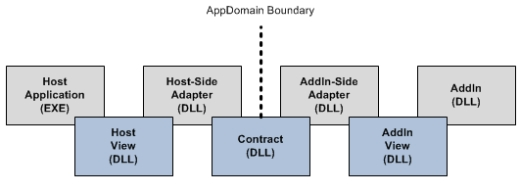
\includegraphics[width=12cm]{System_AddIn_Pipeline.jpg}
    \caption{Схема {\tt Add-in pipeline} в {\tt System.Addin}}
    \label{addin_pipeline-scheme}
\end{figure}

Рассмотрим внутренние компоненты {\tt Add-in pipeline}:

\begin{itemize}

  \item Контракт. Как видно из рисунка, контракт представляет собой интерфейс, <<протокол взаимодействия>> хоста и расширения, и является точкой их соприкосновения;

  \item Далее по обе стороны контракта создаются адаптеры (наследуют {\tt Views}), которые реализуют соответствующие классы представления ({\tt Views}) и оборачивают контракт интерфейсом, который предоставляет {\tt view};

  \item Классы-представления. Они являются соответствующими представлениями типов и методов, которые используются при взаимодействии хоста и расширения.

\end{itemize}

На рисунке \ref{addin_multiple-scheme} представлена схема взаимодействия хост-приложения и плагинов при помощи {\tt Add-in pipeline}.

\begin{figure}[!h]
    \centering
    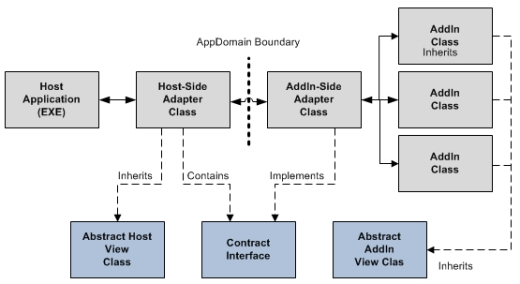
\includegraphics[width=12cm]{System_AddIn_Multiple.jpg}
    \caption{Схема взаимодействия хост-приложения с несколькими плагинами через {\tt Add-in pipeline} в {\tt System.Addin}}
    \label{addin_multiple-scheme}
\end{figure}

Стоит также отметить, что архитектура накладывает некоторые ограничения:
\begin{itemize}

  \item Каждый сегмент из конвейера представляет собой отдельную сборку. Представления можно объединить в одну сборку, но только при условии такого же объединения адаптеров;

  \item {\tt Addin}-ы, адаптеры и контракты должны быть публичны и помечены специальными атрибутами;

  \item Требуется соблюдение жёсткой структуры папок, которая должна строго соблюдаться для нормального функционирования конвейера;

  \item Так как наиболее типичным является сценарий с активацией расширения в отдельном домене, то при проектировании не стоит забывать о том, что пересекающие границы доменов(в качестве параметров или возвращаемых значений) объекты должны быть сериализуемы.

\end{itemize}

\subsubsection{Mono.AddIns}

Эта платформа представляет из себя независимую свободную попытку реализации платформы {\tt Managed AddIn Framework} под {\tt Mono}~\cite{mono-addins-website}.
{\tt Mono.Addins} --- это универсальная платформа для создания расширяемых приложений и самих плагинов для таких приложений. Платформа была разработана  как для работы с небольшими приложениями (с простейшими механизмами расширения), так и для работы с крупными системами, расширяемость которых заложена в дизайн и играет одну из ключевых ролей.

Основные особенности платформы {\tt Mono.Addins}:
\begin{itemize}
  \item поддержка описания плагина с помощью пользовательских атрибутов (для простых расширений) либо с помощью {\tt XML}-манифеста (в более сложных случаях);
  \item поддержка расширений-метаданных и расширений, содержащих только данные;
  \item поддержка иерархии расширений, в которой один плагин может зависеть от других;
  \item <<ленивая>> загрузка плагинов;
  \item использование одного набора установленных расширений несколькими приложениями;
  \item динамическая активация и деактивация расширения в процессе выполнения основного приложения;
  \item разработка расширяемых библиотек;
  \item локализация расширения;
  \item наличие {\tt API} для доступа к описанию расширений, за счёт чего возможно создание инструментов для разработки и документирования плагинов;
  \item наличие инструментов для установки и управления плагинами.
\end{itemize}

\subsubsection{Другие разработки}

\TODO{Сюда пишем  про то, что есть много учебных проектов и SDA}

\subsubsection{Выводы}

Рассмотренные выше платформы теоретически могут применяться для разработки расширяемых приложений, однако интеграция их в готовое приложение крайне сложна, если вообще возможна. Этот недостаток делает крайне неудобным использование перечисленных платформ в рамках задачи по портированию расширяемых приложений. Так же стоит упомянуть о том, что многие рассмотренные платформы пребывают на стадиях альфа- или бета- тестирования, что делает их применение не целесообразным в больших программных комплексах. Однако, основные принципы построения существующих платформ для интеграции поддержки расширений с успехом может быть использован для проектирования собственной платформы.

\subsection{Сравнительный анализ продуктов}

Выше были рассмотрены различные средства для поддержки скриптов либо плагинов. Эти средства, несмотря на их различия имеют массу схожих параметров и признаков, так как в них, как правило, заложены одни и те же идеи. Поэтому, в рамках текущей задачи по реализации платформы для поддержки и скриптов и плагинов имеет смысл сравнивать между собой оба класса средств.

\subsubsection{Критерии сравнения}
\label{sec:comp_criteria}
На основании требований к программному продукту были сформулированы следующие критерии оценки существующих разработок. Критерии приведены в порядке убывания их значимости, хотя удовлетворение всем этим критериям является критичным для реализации замены VBA в рамках проекта по портированию приложения с COM на .NET. Критерии подразумевают различные варианты соответствия. Некоторые – бинарный ответ (удовлетворяет, либо нет), некоторые – предлагают провести сравнительную оценку степени соответствия, некоторые определяют вероятность или прогноз.

\begin{enumerate}
\item Тип продукта (Платформа, Библиотека, Язык, и т.д.);
\item Статус релиза;
\item Возможность реализации расширения конечным пользователем;
\item Наличие IDE для создания кода расширения;
\item Возможность отладки расширения;
\item Сложность интеграции в готовое приложение;
\item Открытость исходного кода;
\item Скрипты или плагины?;
\item Отслеживание зависимостей расширений;
\item Лицензирование.
\end{enumerate}

Следующий этап – создание сравнительной таблицы, которая будет показывать насколько тот или иной продукт удовлетворяет поставленной задаче. Для того, чтобы продукт было возможно использовать, необходимо полное или почти полное удовлетворение всем имеющимся критериям.

\pagebreak

\begin{landscape}

\begin{table}[H]
  \caption{Сравнительная таблица технологий, подходов и платформ для создания расширяемых и/или автоматизируемых приложений}
  \label{tabular:tech_compare_tab}
  \begin{center}
  \begin{tabular}{|p{4.5cm}|c|c|c|c|c|c|c|c|c|}
  
    \hline
      Критерий &
      MEF &
      Al Platform &
      Plux.NET &
      VBA &
      VSTA/VSTO &
      System.Addin &
      Mono.AddIns &
      IronPython &
      SDA \\
    \hline
      Тип продукта &
      FW &
      FW &
      FW &
      Lang &
      FW &
      Lib &
      Lib &
      Lang &
      Tech \\
    \hline
      Статус релиза &
      A &
      B &
      B &
      S &
      S &
      S &
      S &
      S &
      S \\
    \hline
      Для конечного пользователя? &
      Нет &
      Нет &
      Нет &
      Да &
      Да &
      Нет &
      Нет &
      Да &
      Нет \\
    \hline
      Наличие IDE для создания кода расширения &
      Нет &
      Нет &
      Нет &
      Да &
      Да &
      Нет &
      Нет &
      Нет &
      Нет \\
    \hline
      Возможность отладки расширения &
      Нет &
      Нет &
      Нет &
      Да &
      Да &
      Нет &
      Нет &
      Да &
      Нет \\
    \hline
      Сложность интеграции в готовое приложение &
      ? &
      ? &
      ? &
      + &
      + &
      ? &
      ? &
      + &
      - \\
    \hline
      Открытость исходного кода &
      Нет &
      Нет &
      Нет &
      Нет &
      Нет &
      Нет &
      Да &
      Да &
      Да \\
    \hline
      Скрипты или плагины? &
      Плагин &
      Плагин &
      Плагин &
      Скрипт &
      Оба &
      Плагин &
      Плагин &
      Скрипт &
      Плагин \\
    \hline
      Отслеживание зависимостей расширений &
      Да &
      Да &
      Да &
      Нет &
      Нет &
      Нет &
      Нет &
      Нет &
      Да \\
    \hline
      Лицензирование &
      MPL &
      PR &
      FreeWare &
      EULA &
      EULA &
      EULA &
      MIT &
      GPL &
      GPL \\
    \hline
    
  \end{tabular}
  \end{center}
\end{table}

\end{landscape}

\subsubsection{Условные обозначения}

{\bf Тип продукта}

\begin{itemize}
	\item FW: (Framework) Готовая платформа для внедрения комплексной поддержки расширений в разрабатываемое приложение.
	\item Lib: (Library) Библиотека, сторонняя, или встроенная в платформу .NET, предоставляющая инструменты реализации процессов и механизмов, необходимых для организации работы с расширениями или скриптами.
	\item Lang: Язык программирования (скриптовый), имеющий возможность простой интеграции в приложение как средство реализации макросов. 
	\item Tech: Технология, позволяющая решать задачу интеграции возможностей расширяемости, но не являющаяся платформой.
\end{itemize}

{\bf Статус релиза}

\begin{itemize}
	\item A: (Alpha) Нестабильная версия для внутреннего тестирования. Может быть использована в реальном проекте с рядом допущений и рисков.
	\item В: (Beta) Нестабильная версия для публичного тестирования. Может быть использована в реальном проекте с рядом допущений и рисков.
	\item S: (Stable release) Стабильная RTM версия, может быть использована без ограничений.
\end{itemize}

{\bf Сложность интеграции в готовое приложение}

\begin{itemize}
	\item +: Интеграция в готовое приложение возможна, но требует значительных усилий. Относится, как правило, к средствам интеграции макросов.
	\item -: Интеграция в готовое приложение невозможна.
	\item ?: Сложность интеграции сложно оценить, так как она сильно зависит от архитектуры приложения и требуемой глубины интеграции. Относится, как правило, к платформам для поддержки расширений.
\end{itemize}

{\bf Лицензирование}

\begin{itemize}
	\item MPL: Mozilla Public License
	\item FreeWare: Бесплатное ПО, распространяемое без исходного кода.
	\item PR: Проприетарная лицензия. При приобретении Al Platform частично предоставляется исходный код.
	\item GPL: General Public License
	\item EULA: Пользовательское соглашение компании Microsoft.
\end{itemize}

\subsection{Выводы}

Большинство доступных инструментов, платформ и библиотек для создания расширений не решают поставленную задачу, а именно предоставление создания, распространения и отладки расширений конечному пользователю приложения, либо решают ее не полностью. Это происходит из-за устоявшегося разделения сфер внедрения и сценариев использования инструментов расширения и автоматизации. Наиболее подходящей выдвинутым критериям оказалась VSTA от компании Microsoft.

Так же интерес вызывает технология {\it SDA} и продукт {\it SharpDevelop}. Но сам по себе, этот вариант не решает поставленную задачу, требуется разработка собственной платформы управления пользовательскими расширениями. И именно {\it SDA} будет использована в качестве основной технологии в этой разработке. Так же, в рамках исследовательской работы были рассмотрены наиболее распространенные и эффективные подходы к реализации подобных приложений на примере существующих платформ для создания расширений. В дальнейшей разработке я постараюсь применить эти подходы <<как есть>>, адаптировать под особенности конкретной реализации или даже улучшить их.

Проанализировав различные программные продукты можно сделать вывод о неуниверсальности предлагаемых решений. На текущий момент понятия <<плагин>> и <<скрипт>> сильно отдалены друг от друга, и для того чтобы добавить возможность использования обоих видов расширений, приходится внедрять в приложение различные технологии и механизмы, не связанные друг с другом. Это усложняет разработку и использование программных продуктов. Однако, из-за схожих механизмов взаимодействия с приложением у плагинов и скриптов, интересным решением будет объединение этих понятий и реализация универсальной платформы для работы с обоими видами расширений.

\pagebreak
